\subsection{État du jeu}

\subsection{Configuration initiale du jeu}
\begin{itemize}
        \item 
        Grille modulable selon le niveau (surface différente)
        \item 
        Bonbons de couleurs (jaune rouge vert bleu orange)
        \item 
        Bonbons spéciaux (explosion horizontale/verticale, poisson, bombe multicolore, bombe à retardement, bombe colorante)
        \item 
        bloqueurs (bloque présence bonbon, bloque le bonbon)
        \item 
        Nombre de coups pour réussir / temps
        \item 
        Score
        \item 
        Jauge à remplir pour les étoiles
        \item 
        Objectif à réaliser
\end{itemize}

\subsection{Évolution de l'état du jeu}
\subsubsection{Vérification du déplacement}
Avant de pouvoir échanger deux cases, il faut vérifier plusieurs choses :
\begin{itemize}
	\item
		Le déplacement ne sort pas de la grille
\begin{lstlisting}
caseDestination.x >= 0 && caseDestination.x < tailleGrilleX && caseDestination.y >= 0 && caseDestination.y < tailleGrilleY
\end{lstlisting}
	\item
		Le déplacement ne va pas sur une case non-jouable
\begin{lstlisting}
grille[caseDestination.x][caseDestination.y] != 0 && grille[caseADeplacer.x][caseADeplacer.y] != 0
\end{lstlisting}
	\item
		Les cases sont côtes à côtes (si on clique autre part, ça change la position de la caseADeplacer) :
\begin{lstlisting}
caseADeplacer.x - caseDestination.x == 1 || caseADeplacer.x - caseDestination.x == -1 || ( caseADeplacer.x - caseDestination.x != 1 && caseADeplacer.x - caseDestination.x != -1 && (caseADeplacer.y - caseDestination.y == 1 || caseADeplacer.y - caseDestination.y == -1) )
\end{lstlisting}
	\item
		Le déplacement va créer un alignement de au moins 3 cases identiques : pour cela, on va tout d'abord échanger les deux cases sélectionnées grace à la case temporaire :
\begin{lstlisting}
caseTemporaire = grille[caseDestination.x][caseDestination.y];
grille[caseDestination.x][caseDestination.y] = grille[caseADeplacer.x][caseADeplacer.y];
grille[caseADeplacer.x][caseADeplacer.y] = caseTemporaire;
\end{lstlisting}
		On peut alors commencer la détection des cases à détruire. Si il n'y a aucune case à détruire (lors de la première fois qu'on cherche), il n'y a donc pas de combinaison, on peut alors rééchanger les cases.
\end{itemize}

\begin{figure}[position]
	\center
	\caption{\label{verifDepl} Déplacements}
	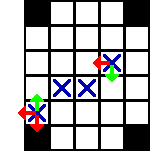
\includegraphics{imgs/verifDepl}
\end{figure}
		
\subsubsection{Détection}	
	
Pour pouvoir détecter toutes les cases à détruire, nous utilisons une autre grille de la même taille que celle contenant les éléments, mais cette nouvelle grille contient des booléens. Chaque case est ainsi associée à un booléen. Si la case doit être détruite, le booléens vaudra vrai.

On va ensuite parcourir la première grille ligne par ligne pour marquer tous les alignements horizontaux puis colonne par colonne pour les combinaisons verticales.

\begin{figure}[position]
	\center
	\caption{\label{Detection} Détection}
	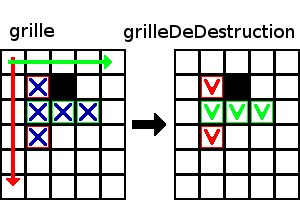
\includegraphics{imgs/Detection}
\end{figure}

Nous avons besoin de quelques nouvelles variables :

\begin{lstlisting}
int couleurTemp; // Couleur temporaire qui va servir pour verifier que plusieurs cases sont identiques
int nbCasesAlignees; // Sert a compter le nombre de cases alignees
\end{lstlisting}

Pour parcourir la grille :

\begin{lstlisting}
for(int j = 0; j < tailleGrilleY; j++)
{
	couleurTemp = grille[0][j]; // La couleur temporaire est egale a la premiere case de la grille
	nbCasesAlignees = 1; // Le nombre de cases alignees est egal a 1 en debut de ligne
	/** Parcours des lignes **/
	for(int i = 0; i < tailleGrilleX; i++)
	{
		if(couleurTemp == grille[i][j]) // Si la couleur temporaire est la meme dans cette case, on incremente nbCasesAlignees
			nbCasesAlignees++;
		else if(nbCasesAlignees >= 3)
		{
			// Si la couleur n'est pas la meme mais qu'on a un alignement, on note dans le deuxieme tableau
			nbCasesAlignees = 1;
			couleurTemp = grille[i][j];
			pasDeCasesADetruire = false;
		}
		else
		{
			nbCasesAlignees = 1;
			couleurTemp = grille[i][j];
		}

		if(i == tailleGrilleX - 1 && nbCasesAlignees >= 3) 
			/* Si on atteind le bord de la grille et qu'on a un alignement de plus de 3,
			on note dans le tableau apres avoir incremente i, pour utiliser la meme fonction de notation dans l'autre tableau. */
	}
} 
\end{lstlisting}
		Pour noter les cases à détruire dans la seconde grille, on peut simplement faire :
\begin{lstlisting}
for(int k = i - nbCasesAlignees; k < i; k++) // On parcours les cases a noter, mais on ne passe pas quand k == i car la case i ne fait pas partie de l'alignement
{
	grilleDeDestruction[k][j] = true;
}
\end{lstlisting}

Il faudra refaire ce processus de détection des alignements verticalement, donc colonne par colonne. Le principe est identique.

\subsubsection{Destruction}

Pour détruire les cases, nous remplaçons les cases à détruire par -1 dans la grille.

\begin{figure}[position]
	\center
	\caption{\label{Destruction} Destruction}
	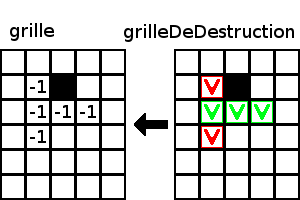
\includegraphics{imgs/Destruction}
\end{figure}

Cela se traduit comme suit :

\begin{lstlisting}
for(int j = 0; j < tailleGrilleY; j++)
{
	for(int i = 0; i < tailleGrilleX; i++)
	{
		if(grilleDeDestruction[i][j] == true)
		{
			grille[i][j] = -1;
			grilleDeDestruction[i][j] = false; // On en profite pour reinitialiser la deuxieme grille qui sert pour la destruction
		}
	}
}
\end{lstlisting}

\subsubsection{Remplacement}

	Afin de remplacer les cases détruites (donc -1 dans la grille), il faut trier la grille de manière à avoir tout les -1 au dessus.
	Il faut tout de même penser aux cases inutilisables (0 dans la grille) qui ne doivent pas être bougées.
	
	Nous allons donc parcourir chaque colonne en partant du bas, et lorsqu'on trouve un -1, nous allons le remplacer par la prochaine case valide (qu'on mettra à -1).
	
\begin{figure}[position]
	\center
	\caption{\label{Remplacement} Remplacement}
	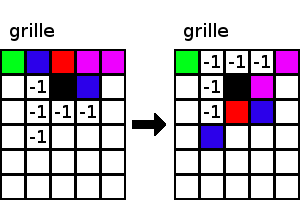
\includegraphics{imgs/Remplacement1}
	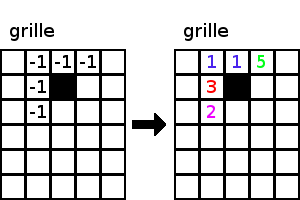
\includegraphics{imgs/Remplacement2}
\end{figure}
	
	Pour une colonne k, nous aurons :
\begin{lstlisting}
int j;
boolean continuer;
for(int i = tailleGrilleY - 1; i >= 0; i--)
{
	if(grille[k][j] == -1)
	{
		j = i;
		continuer = true;
		while(j >= 0 && continuer == true)
		{
			j--;
			if(grille[k][j] != 0 && grille[k][j] != -1) // Si on trouve une case correcte, on remplace
			{
				grille[k][i] = grille[k][j];
				grille[k][j] = -1;
				continuer = false; // On n'a plus besoin de rechercher
			}
		}
	}
}
\end{lstlisting}

	Il faudra faire une boucle pour répliquer ce résonnement à chaque colonne. Notons qu'on pourrais ajouter une condition qui arrêterais la boucle la première fois que le while ne trouve pas de case valide.
	
	Désormais, il ne reste plus qu'à remplacer toutes les cases -1 par un numéro aléatoire 1, 2, 3, 4 ou 5 représentant les différents types de cases.

\begin{lstlisting}
for(int j = 0; j < tailleGrilleY; j++)
{
	for(int i = 0; i < tailleGrilleX; i++)
	{
		if(grille[i][j] == -1;
			grille[i][j] = (int)(Math.random() * 5) + 1;
	}
}
\end{lstlisting}

\subsubsection{Finalement}

Ce processus Détection-Destruction-Remplacement devra être répété jusqu'à ce qu'il n'y ait plus aucune case à détruire.

De plus, un score à atteindre pourra être fixé. Pour cela, chaque destruction de case (quand on les mets à -1) incrémentera d'un certain nombre de points la variable scoreActuel. Le jeu pourra s'arrêter lorsque le score ciblé est atteint.
\begin{lstlisting}
scoreActuel >= scoreCible
\end{lstlisting}

Enfin, il est possible de compter le nombre de coups que le joueur a utilisé. En effet, il suffit de le faire lors de l'échangement des cases. Si cet échange est par la suite annulé, le nombre de coups sera remis à son état d'avant l'échange.